\documentclass[a4paper]{report}
\usepackage[utf8]{inputenc}
\usepackage{hyperref}
\usepackage{a4wide}
\hypersetup{pdftitle={Dotprod},
pdfauthor={João Teixeira, José Ferreira},
colorlinks=true,
urlcolor=blue,
linkcolor=black}
\usepackage{subcaption}
\usepackage[cache=false]{minted}
\usepackage{listings}
\usepackage{booktabs}
\usepackage{multirow}
\usepackage{appendix}
\usepackage{tikz}
\usepackage{authblk}
\usepackage{bashful}
\usepackage{verbatim}
\usepackage{amssymb}
\usepackage{multirow}
\usepackage{mwe}
\usepackage[parfill]{parskip}
\usetikzlibrary{positioning,automata,decorations.markings}
\AfterEndEnvironment{figure}{\noindent\ignorespaces}
\AfterEndEnvironment{table}{\noindent\ignorespaces}

\usepackage{titlesec}

\titleformat{\chapter}[display]
   {\normalfont\large\bfseries}{\chaptertitlename\ \thechapter}{0pt}{\huge}
\titlespacing*{\chapter}{0pt}{0pt}{0pt}

\begin{document}

\title{Advanced Architectures\\Dotprod Implementations and Benchmarking}
\author{João Teixeira (A85504) \and José Filipe Ferreira (A83683)}
\date{\today}

\begin{center}
    \begin{minipage}{0.75\linewidth}
        \centering
        
\includegraphics[width=0.4\textwidth]{images/eng.jpeg}\par\vspace{1cm}
        \vspace{1.5cm}
        \href{https://www.uminho.pt/PT}
        {\color{black}{\scshape\LARGE Universidade do Minho}} \par
        \vspace{1cm}
        \href{https://www.di.uminho.pt/}
        {\color{black}{\scshape\Large Departamento de Informática}} \par
        \vspace{1.5cm}
        \maketitle
    \end{minipage}
\end{center}

\tableofcontents

\pagebreak

\chapter{Introduction}

\chapter{Full characterization of the hardware}
Our team's main laptop is a Lenovo ThinkPad X260. It is powered by a i5-6300U, a
dual-core hyperthreaded skylake cpu.

To get more information related to the CPU's memory hierarchy we used the
command \textit{lstopo} that displays a graphic with information related with
the cache size.
\begin{figure}[H]
    \centering
        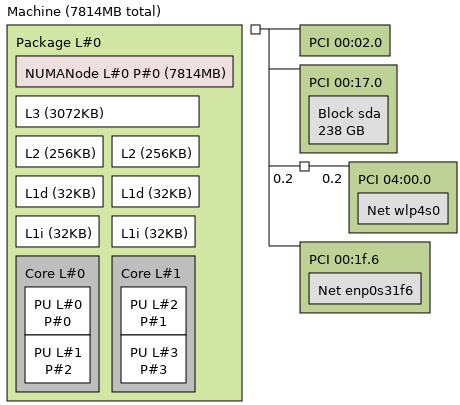
\includegraphics[width=0.5\textwidth]{images/lstopo.png}
        \caption{lstopo graphic}
\end{figure}

As it is visible in the picture above the CPU has 32KiB of L1 cache per core,
256KiB of L2 cache per core and 3072MiB L3 cache. It also has 7814MiB of Random
Access Memory(RAM).

\chapter{Dotprod Implementation}
The dotprod is a mathematical operation between two matrices (A and B) that results in
another matrix (C). To obtain the position (i,j) in the matrix C we need to
multiply each value of the line i in the matrix A with each value of the collum
j of the matrix B and add them.

When programming this behaviour it is commonly used a nested triple for loop
going from 0 to the size of the matrix. Each loop having a different variable
usually i, j and k. The variable i indexes the lines on the A matrix, the j
indexes the columns on the B matrix and the k is the loop that iterates over the
line and column.

\begin{figure}[H]
    \centering
        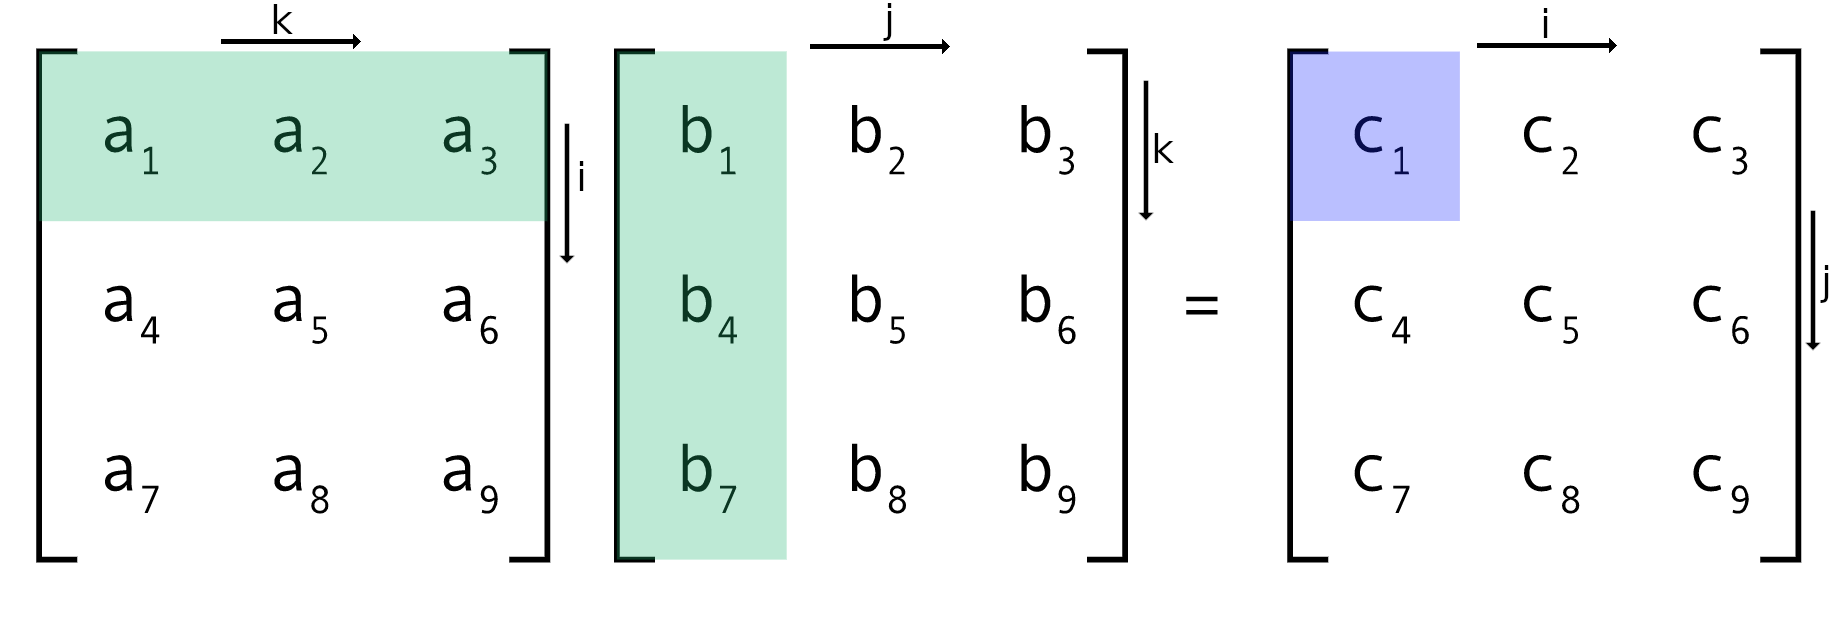
\includegraphics[width=0.7\textwidth]{images/matrix_mult.png}
        \caption{Dotprod Diagram}
\end{figure}

The first implementation of the algoritm had the nested loop in the order
\textbf{i-j-k}. However, this order can be altered whitout having to change the
content of the loop. Therefore, in order to measure diferences in performance
two other options were created: \textbf{i-k-j} and \textbf{j-k-i}. After
analizing all the created algoritms we realized that the way the matrices were
indexed differed between implementation. In some they were acessed by collumn
and others by line.

While accessing a matrix line by line explores cache locality and decreases
cache misses, accessing a matrix collumn by collumn increases cache misses due
to a lower cache locality. Therefore, in order to mitigate the penalty of
accesing the matrices collum by collum two more algorithms were created:
\textbf{i-j-k trans} that transposes the matrix B before computing the
dotprod; \textbf{j-k-i trans} that transposes the matrices A and B before
calculating the dotprod and transposes the matrix C after ccomputing.

This results in the followin patterns of access depending on the algorithm:

\begin{table}[H]
\centering
\begin{tabular}{|l|l|l|l|}
\hline
                     & A       & B       & C       \\ \hline
\textbf{i-j-k}       & line    & collumn & line    \\ \hline
\textbf{i-j-k trans} & line    & line    & line    \\ \hline
\textbf{i-k-j}       & line    & line    & line    \\ \hline
\textbf{j-k-i}       & collumn & collumn & collumn \\ \hline
\textbf{j-k-i trans} & line    & line    & line    \\ \hline
\end{tabular}
\caption{matrices access based on loop order}
\end{table}

In order to explore even more cache locality another version of the algorithm
was created that uses block optimization. In this version of the algorithm we
used the access order of \textbf{i-j-k} while also transposing the matrix B in
order to be able to access it line by line.

In this version, only part of a line of A, a block of B and part of a line of C
is kept in cache at any given time. The line from A is multiplied by the block
from B in order to populate the line in C. And after this calculation is done,
another section of A is fetched that is multiplied by the same block in B
in order to compute another section of a line from C.

\begin{figure}[H]
    \centering
        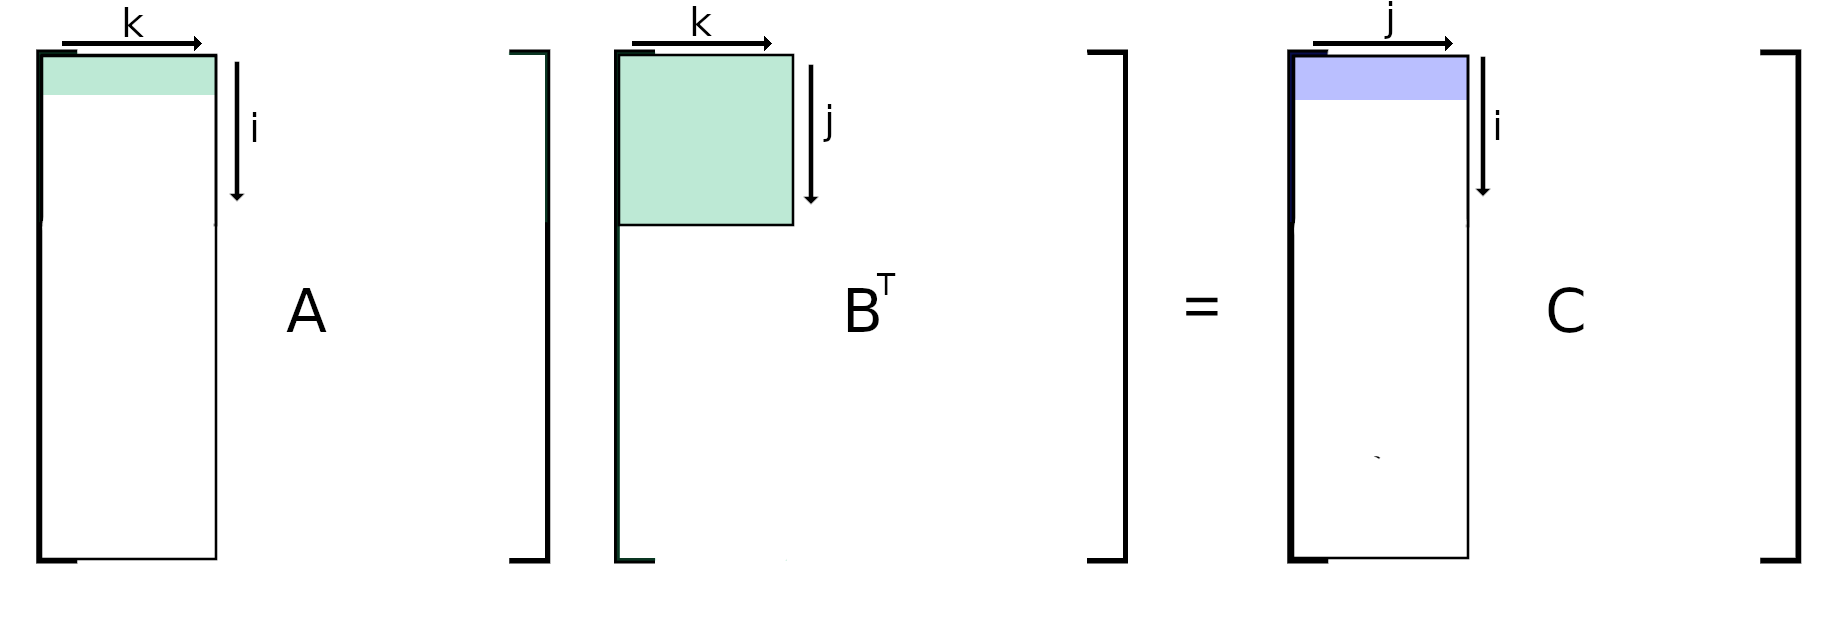
\includegraphics[width=0.7\textwidth]{images/matrix_mult_block.png}
        \caption{Dotprod with Block Optimization}
\end{figure}

After creating a working dotprod implementation with block optimization we
decided to apply the vectozition flags to the compilation and analize the
compiler output in order to check if the code was vectorizable. Due to a Read
after write data dependency minor tweaks had to be applied to the code in order
for it to vectorize successfully.

Finally this version of the dotprod with block optimization and vectorization
was modified to run efficiently on all cores of a multicore device making use of
the OpenMP.



\chapter{Dotprod Benchmarking}
In order to properly benchmark the different algorithms created and compare them
we choose to collect data with PAPI and \textit{sys/time.h}. The full list of
counters available in the used system is on the Appendix \ref{A:papi_avail}. From
this list we choose to use the following PAPI counters: EVENT PAPI\_L1\_TCM, EVENT
PAPI\_L2\_TCM, EVENT PAPI\_L3\_TCM, EVENT PAPI\_LD\_INS, EVENT PAPI\_SR\_INS and
EVENT PAPI\_TOT\_INS. With this set of counters we can validate the theory that
different algorithms have different cache misses and memory access.

To also benchmark the impact of different sizes of matrices we choose four
different sizes. The smaller one fits in L1 cache, then L2 cache, then L3 cache
and finally the biggest on requires significant access to RAM. Based on the CPU
used for benchmarking the following table was created:

\begin{table}[H]
\centering
\begin{tabular}{|l|l|l|l|l|}
\hline
           & L1 data & L2 data & L3 data  & RAM                    \\ \hline
cache size & 32768   & 262144  & 31457280 & \textgreater{}31457280 \\ \hline
max size   & 52      & 147     & 1619     & \textgreater{}1619     \\ \hline
used size  & 40      & 120     & 1500     & 4000                   \\ \hline
\end{tabular}
\caption{Matrix sizes used for benchmarking}
\end{table}

For the tests, the matrix A was filled with random numbers and the matrix B was
filled with ones. This way, AxB results in a matrix where all column have the
same value and BxA results in a matrix where all lines have the same value. This
property was used to assert if all the variations of the algorithm were producing
the correct results. After each test the cache was cleared to ensure all the
tests used a cold cache. To reduce the outliers, the time measurements were
performed 8 times using a K-best scheme with K=3 and a tolerance of 5\%.

\begin{table}[H]
\centering
\begin{tabular}{|l|l|l|l|l|}
\hline
            & 40x40 & 120x120 & 1500x1500 & 4000x4000 \\ \hline
i-j-k       & 66    & 1733    & 4239493   & 177553349 \\ \hline
i-j-k trans & 94    & 1698    & 3223331   & 71675215  \\ \hline
i-k-j       & 71    & 1718    & 3194044   & 61695968  \\ \hline
j-k-i       & 72    & 1744    & 8596300   & 324751067 \\ \hline
\textit{j-k-i trans} & \textit{69}    & \textit{1375}    & \textit{2273077}   &
\textit{45375529}  \\ \hline
\end{tabular}
\caption{Execution time for non-blocking sequential algorithms (time in $\mu$s)}
\end{table}

\begin{table}[H]
\centering
\begin{tabular}{|l|l|l|l|l|}
\hline
            & 40x40   & 120x120 & 1500x1500 & 4000x4000 \\ \hline
i-j-k       & .001321 & .000057 & .000582   & .781009   \\ \hline
i-j-k trans & .001911 & .000105 & .000308   & .084568   \\ \hline
i-k-j       & .027150 & .007252 & .000259   & .030864   \\ \hline
j-k-i       & .036501 & .008403 & .001570   & .785903   \\ \hline
\textit{j-k-i trans} & \textit{.034159} & \textit{.008555} & \textit{.000902}
                     & \textit{.053824}   \\ \hline
\end{tabular}
\caption{Ram access per total instructions (\%)}
\end{table}

\begin{table}[H]
\centering
\begin{tabular}{|l|l|l|l|l|l|}
\hline
\multicolumn{2}{|l|}{}            & 40x40 & 120x120 & 1500x1500 & 4000x4000 \\ \hline
\multirow{3}{*}{i-j-k}       & L1 & .2360 & 2,1902  & 35.5386   & 34.4700   \\ \cline{2-6}
                             & L2 & .0762 & .0237   & 2.3420    & 34.4019   \\ \cline{2-6}
                             & L3 & .0025 & .0001   & .0016     & 2.0842    \\ \hline
\multirow{3}{*}{i-j-k trans} & L1 & .1865 & 2.0801  & 2.0981    & 2.1194    \\ \cline{2-6}
                             & L2 & .0902 & .0294   & .0532     & .7009     \\ \cline{2-6}
                             & L3 & .0664 & .0196   & .0015     & .2712     \\ \hline
\multirow{3}{*}{j-k-i}       & L1 & .1411 & 1.9620  & 50.0075   & 50.1961   \\ \cline{2-6}
                             & L2 & .0873 & .0273   & 9.6299    & 50.1126   \\ \cline{2-6}
                             & L3 & .0709 & .0173   & .0031     & 1.5741    \\ \hline
\multirow{3}{*}{\textit{j-k-i trans}} & \textit{L1} & \textit{.6037} & \textit{7.9182}  & \textit{8.4272}    & \textit{8.5532}    \\ \cline{2-6}
                                      & \textit{L2} & \textit{.3874} & \textit{.1204}   & \textit{.2507}     & \textit{6.4841}    \\ \cline{2-6}
                                      & \textit{L3} & \textit{.3270} & \textit{.0831}   & \textit{.0087}     & \textit{2.9880}    \\ \hline
\end{tabular}
\caption{global miss rate for algoritms that benefited from transposing}
\end{table}

\begin{table}[H]
\centering
\begin{tabular}{|l|l|l|l|}
\hline
          & i-j-k trans & i-j-k trans + block & speedup \\ \hline
4000x4000 & 71675215    & 64385275            & 1.1132  \\ \hline
\end{tabular}
\caption{time comparison of block optimisation (time in $\mu$)}
\end{table}

\begin{table}[H]
\centering
\begin{tabular}{|l|l|l|l|}
\hline
        & i-j-k trans & i-j-k trans + block + vec & speedup \\ \hline
40x40   & 94          & 71                        & 1.3239  \\ \hline
120x120 & 1698        & 1523                      & 1.1149  \\ \hline
\end{tabular}
\caption{time comparison of block optimization with vectorization (time in
$\mu$)}
\end{table}

\begin{table}[H]
\centering
\begin{tabular}{|l|l|l|l|}
\hline
          & i-j-k trans & i-j-k trans + block + vec + OpenMP & speedup \\ \hline
4000x4000 & 71675215    & 2407551                            & 29.7710 \\ \hline
\end{tabular}
\caption{time comparison of block optimization with vectorization and OpenMP (time in
$\mu$)}
\end{table}

\chapter{Conclusions}

\appendix

\chapter{Available papi counters}\label{A:papi_avail}
\verbatiminput{papi_avail_-a.txt}

\end{document}
